\section{Thiết lập thực nghiệm và Kịch bản đánh giá trôi dạt khái niệm}

Thực nghiệm được thiết lập nhằm đánh giá khả năng học trực tuyến và độ ổn định cấu trúc của thuật toán EAGNG trên dòng dữ liệu khuyết tật màn hình điện thoại. Toàn bộ kịch bản kiểm thử được xây dựng theo tiêu chuẩn kiểm tra công nghiệp, bảo đảm tính thống nhất về môi trường tính toán, phương pháp trích xuất đặc trưng và hệ thống chỉ số đo lường.

\subsection{Môi trường thực nghiệm và Cơ sở hạ tầng tính toán}
\label{subsec:moi_truong_thuc_nghiem}

Môi trường phần cứng tính toán đóng vai trò quyết định đến độ tin cậy của việc đo lường thời gian xử lý trực tuyến. Hệ thống thực nghiệm được triển khai trên máy tính cấu hình bao gồm vi xử lý Intel Core i5-13400F, bộ nhớ truy cập ngẫu nhiên 16 gigabyte và bộ xử lý đồ họa NVIDIA GeForce RTX 3060 dung lượng 12 gigabyte. Cơ sở hạ tầng phần cứng này bảo đảm năng lực tính toán song song cho quá trình trích xuất đặc trưng và mô phỏng dòng dữ liệu thời gian thực.

Nền tảng phần mềm được xây dựng trên hệ điều hành Windows 11 nhằm duy trì tính đồng nhất trong quá trình thu thập dữ liệu. Môi trường tính toán sử dụng thư viện PyTorch phiên bản 2.13.0 kết hợp với thư viện Scikit-Learn phiên bản 1.9.0 cho các tác vụ xử lý ma trận và tính toán chỉ số phân cụm. Cấu hình chi tiết của cơ sở hạ tầng tính toán được tổng hợp trong Bảng \ref{tab:hardware_software_config}.

\begin{table}[htbp]
\centering
\caption{Thống kê thông số môi trường phần cứng và phần mềm thực nghiệm.}
\label{tab:hardware_software_config}
\begin{tabular}{|l|l|}
\hline
Thành phần hệ thống & Thông số kỹ thuật \\ \hline
Vi xử lý & Intel Core i5-13400F \\ \hline
Bộ nhớ ngẫu nhiên RAM & 16 GB DDR4 \\ \hline
Bộ xử lý đồ họa GPU & NVIDIA GeForce RTX 3060 12 GB \\ \hline
Hệ điều hành & Windows 11 \\ \hline
Môi trường phần mềm & PyTorch 2.13.0, Scikit-Learn 1.9.0 \\ \hline
\end{tabular}
\end{table}

Hệ thống chỉ số đánh giá được thiết lập bao quát cả ba khía cạnh bao gồm chất lượng phân cụm, độ ổn định cấu trúc tô-pô và hiệu năng thời gian thực. Chất lượng phân cụm trực tuyến được định lượng thông qua ba chỉ số độc lập là chỉ số Rand điều chỉnh, thông tin tương hỗ chuẩn hóa và độ tinh khiết phân cụm.

Chỉ số Rand điều chỉnh đo lường mức độ tương đồng giữa kết quả phân cụm thu được và nhãn thực tế của dữ liệu, loại bỏ yếu tố trùng khớp ngẫu nhiên \cite{hubert1985comparing}. Công thức \ref{eq:ari} biểu diễn phép tính chỉ số Rand điều chỉnh:
\begin{equation}
ARI = \frac{\sum_{ij} \binom{n_{ij}}{2} - \left[ \sum_i \binom{a_i}{2} \sum_j \binom{b_j}{2} \right] / \binom{n}{2}}{\frac{1}{2} \left[ \sum_i \binom{a_i}{2} + \sum_j \binom{b_j}{2} \right] - \left[ \sum_i \binom{a_i}{2} \sum_j \binom{b_j}{2} \right] / \binom{n}{2}}
\label{eq:ari}
\end{equation}
Trong Công thức \ref{eq:ari}, ký hiệu $n_{ij}$ đại diện cho số lượng mẫu dữ liệu thuộc cùng cụm thứ $i$ và nhãn thực tế thứ $j$, ký hiệu $a_i$ thể hiện tổng số mẫu trong cụm $i$, ký hiệu $b_j$ đại diện cho tổng số mẫu mang nhãn $j$, và ký hiệu $n$ biểu thị tổng số mẫu dữ liệu trong dòng học tính đến thời điểm đánh giá.

Thông tin tương hỗ chuẩn hóa đánh giá lượng thông tin chia sẻ giữa cấu trúc phân cụm của mô hình và tập nhãn thực tế \cite{strehl2002cluster}. Giá trị thông tin tương hỗ chuẩn hóa được xác định theo Công thức \ref{eq:nmi}:
\begin{equation}
NMI(Y, C) = \frac{2 \cdot I(Y; C)}{H(Y) + H(C)}
\label{eq:nmi}
\end{equation}
Trong Công thức \ref{eq:nmi}, ký hiệu $I(Y; C)$ biểu thị lượng thông tin tương hỗ giữa tập nhãn thực tế $Y$ và tập cụm dự đoán $C$, trong khi ký hiệu $H(Y)$ và $H(C)$ đại diện cho độ dư thừa thông tin của tập nhãn thực tế và tập cụm thu được.

Độ tinh khiết phân cụm đo tỷ lệ phần trăm mẫu dữ liệu thuộc về lớp chiếm ưu thế nhất trong mỗi cụm thu được. Phép tính độ tinh khiết phân cụm được mô tả cụ thể trong Công thức \ref{eq:purity}:
\begin{equation}
Purity(Y, C) = \frac{1}{N} \sum_{k} \max_{j} |c_k \cap y_j|
\label{eq:purity}
\end{equation}
Trong Công thức \ref{eq:purity}, ký hiệu $N$ biểu thị tổng số mẫu dữ liệu xử lý, ký hiệu $c_k$ đại diện cho tập hợp các mẫu trong cụm thứ $k$, và ký hiệu $y_j$ đại diện cho tập hợp các mẫu có nhãn thực tế thứ $j$.

Mức độ ổn định cấu trúc tô-pô và khả năng kháng hiện tượng quên thảm họa được đo lường thông qua độ dời Euclid cấp hai trung bình của tập nút mạng qua các bước cập nhật dòng dữ liệu. Công thức \ref{eq:displacement} xác định độ dời của tập nút:
\begin{equation}
\Delta W = \frac{1}{|V_t|} \sum_{v \in V_t} \min_{u \in V_{t-1}} \|w_v^{(t)} - w_u^{(t-1)}\|_2
\label{eq:displacement}
\end{equation}
Trong Công thức \ref{eq:displacement}, ký hiệu $V_t$ đại diện cho tập hợp nút mạng tại bước thời gian $t$, ký hiệu $V_{t-1}$ đại diện cho tập hợp nút tại bước thời gian liền trước, ký hiệu $w_v^{(t)}$ biểu diễn véc-tơ trọng số của nút $v$ ở thời điểm $t$, và ký hiệu $w_u^{(t-1)}$ đại diện cho véc-tơ trọng số của nút $u$ ở thời điểm $t-1$.

Hiệu năng xử lý thời gian thực được định lượng thông qua chỉ số thời gian nhịp sản xuất trung bình trên mỗi mẫu dữ liệu. Phép tính thời gian nhịp sản xuất được thiết lập theo Công thức \ref{eq:takttime}:
\begin{equation}
Takt = \frac{T_{total}}{N_{samples}} \times 1000
\label{eq:takttime}
\end{equation}
Trong Công thức \ref{eq:takttime}, ký hiệu $T_{total}$ biểu thị tổng thời gian tích lũy dành cho quá trình cập nhật mô hình tính bằng giây, ký hiệu $N_{samples}$ đại diện cho số lượng mẫu đã xử lý, và giá trị $Takt$ trả về đơn vị mili-giây trên một mẫu.

\subsection{Cấu hình tham số thực nghiệm và thuật toán EAGNG}
\label{subsec:cau_hinh_tham_so}

Tập hợp các tham số thực nghiệm được thiết lập dựa trên kết quả thăm dò kiểm thử nhằm bảo đảm sự cân bằng giữa độ chính xác phân cụm và tốc độ xử lý thời gian thực. Các tham số hệ thống được phân chia thành ba nhóm chức năng chính bao gồm (i) nhóm tham số trích xuất đặc trưng và mô hình mã hóa tự động, (ii) nhóm tham số phát hiện bất thường ngoại tuyến, và (iii) nhóm tham số điều khiển tiến trình học động của thuật toán EAGNG.

Trong nhóm tham số trích xuất đặc trưng, ảnh bề mặt màn hình điện thoại được chuẩn hóa về kích thước $128 \times 128$ pixel. Cửa sổ tính toán bản đồ độ hỗn loạn cục bộ sử dụng kích thước $9 \times 9$ pixel với bán kính phần tử cấu trúc dạng đĩa bằng $4$ pixel. Mô hình mã hóa tự động nén đặc trưng bốn kênh về véc-tơ không gian ẩn có chiều $d = 64$. Quá trình huấn luyện mô hình mã hóa tự động được thực hiện với tốc độ học $\eta_{ae} = 10^{-3}$, kích thước lô dữ liệu $B = 64$ và số chu kỳ huấn luyện $E_{ae} = 10$.

Trong nhóm tham số phát hiện bất thường ngoại tuyến, mô hình biểu diễn phân phối sản phẩm đạt chuẩn được huấn luyện trong $10$ chu kỳ. Ngưỡng phân định sản phẩm bất thường dựa trên quy tắc ba lần độ lệch chuẩn với hệ số $\lambda_{\sigma} = 3{,}0$. Bộ nhớ đệm dành cho các mẫu dữ liệu khuyết tật phát sinh được thiết lập với dung lượng lưu trữ tối đa $S_{buf} = 1000$ mẫu.

Nhóm tham số điều khiển thuật toán EAGNG quy định các cơ chế cập nhật cấu trúc đồ thị và thích ứng trực tuyến. Đồ thị nơ-ron có giới hạn số lượng nút tối đa $N_{max} = 500$ nút và tuổi thọ tối đa của cạnh nối được thiết lập $a_{max} = 50$ bước thời gian. Chu kỳ sinh nút mới theo mức tích lũy sai số được định cấu hình sau mỗi $\lambda = 50$ bước lặp với hệ số chia sai số nút $\alpha = 0{,}5$ và hệ số suy giảm sai số toàn cục $\beta = 0{,}005$. Tốc độ học của nút chiến thắng và các nút lân cận lần lượt nhận giá trị $e_b = 0{,}1$ và $e_n = 0{,}001$.

Các cơ chế cải tiến chuyên biệt trong thuật toán EAGNG được điều khiển bởi các tham số không gian và thời gian. Bán kính quét vùng dữ liệu mới được thiết lập $R_{scan} = 10{,}0$, đòi hỏi tối thiểu $K_{spawn} = 10$ mẫu trong bộ đệm để kích hoạt tiến trình sinh nút và huấn luyện cục bộ trong $E_{local} = 20$ chu kỳ với chu kỳ chèn nút cục bộ $\lambda_{local} = 10$. Giới hạn mật độ cục bộ sử dụng khoảng cách tối thiểu $d_{min} = 5{,}0$ nhằm ngăn ngừa hiện tượng phân mảnh vùng biểu diễn. Hệ số suy giảm tốc độ học theo thời gian sử dụng hằng số thời gian $\tau = 1000$ bước lặp. Ngưỡng giao thoa diện tích giữa các cụm để quyết định nối cạnh được ấn định ở mức $T_{overlap} = 0{,}65$. Bảng \ref{tab:eagng_parameters} tổng hợp chi tiết toàn bộ tham số cài đặt trong thực nghiệm.

\begin{table}[htbp]
\centering
\caption{Tổng hợp giá trị cài đặt các tham số mô hình và thuật toán EAGNG trong thực nghiệm.}
\label{tab:eagng_parameters}

\renewcommand{\arraystretch}{1.15}
\setlength{\tabcolsep}{5pt}

\begin{tabularx}{\textwidth}{|l|c|c|X|}
\hline
Nhóm tham số & Ký hiệu & Giá trị & Ý nghĩa kỹ thuật \\ \hline

Trích xuất đặc trưng 
& - & $128 \times 128$ 
& Kích thước ảnh chuẩn hóa (pixel) \\ \hline

Cửa sổ entropy 
& - & $9 \times 9$ 
& Kích thước cửa sổ độ hỗn loạn (pixel) \\ \hline

Không gian ẩn 
& $d$ & $64$ 
& Số chiều véc-tơ biểu diễn ẩn \\ \hline

Tốc độ học mã hóa 
& $\eta_{ae}$ & $10^{-3}$ 
& Tốc độ học của mô hình Autoencoder \\ \hline

Lô huấn luyện 
& $B$ & $64$ 
& Kích thước lô dữ liệu Autoencoder \\ \hline

Ngưỡng bất thường 
& $\lambda_{\sigma}$ & $3{,}0$ 
& Hệ số ngưỡng phân định $3\sigma$ \\ \hline

Sức chứa bộ đệm 
& $S_{buf}$ & $1000$ 
& Số mẫu khuyết tật tối đa trong bộ đệm \\ \hline

Số nút tối đa 
& $N_{max}$ & $500$ 
& Giới hạn số nút tối đa của đồ thị \\ \hline

Tuổi thọ cạnh 
& $a_{max}$ & $50$ 
& Tuổi thọ tối đa của cạnh nối giữa các nút \\ \hline

Chu kỳ chèn nút 
& $\lambda$ & $50$ 
& Tần suất kiểm tra sinh nút theo sai số \\ \hline

Hệ số chia sai số 
& $\alpha$ & $0{,}5$ 
& Tỷ lệ phân chia sai số khi sinh nút mới \\ \hline

Suy giảm sai số 
& $\beta$ & $0{,}005$ 
& Tỷ lệ suy giảm sai số toàn cục \\ \hline

Tốc độ học nút chính 
& $e_b$ & $0{,}1$ 
& Tốc độ học của nút chiến thắng \\ \hline

Tốc độ học lân cận 
& $e_n$ & $0{,}001$ 
& Tốc độ học của các nút lân cận \\ \hline

Bán kính quét vùng 
& $R_{scan}$ & $10{,}0$ 
& Ngưỡng khoảng cách nhận diện vùng mới \\ \hline

Số mẫu sinh nút 
& $K_{spawn}$ & $10$ 
& Mẫu tối thiểu trong đệm để tạo nút mới \\ \hline

Khoảng cách mật độ 
& $d_{min}$ & $5{,}0$ 
& Ngưỡng khoảng cách mật độ tối thiểu \\ \hline

Hằng số thời gian 
& $\tau$ & $1000$ 
& Hằng số thời gian giảm tốc độ học \\ \hline

Ngưỡng giao thoa 
& $T_{overlap}$ & $0{,}65$ 
& Ngưỡng tỷ lệ giao thoa để nối cạnh \\ \hline

\end{tabularx}

\end{table}

\subsection{Kịch bản dòng dữ liệu khuyết tật liên tục}
\label{sec:4_1_2_data_stream_scenario}

Bộ dữ liệu thực nghiệm được xây dựng bao gồm $3000$ ảnh mô phỏng các dạng khuyết tật bề mặt màn hình điện thoại trong môi trường kiểm tra công nghiệp. Ảnh thu nhận ban đầu đạt độ phân giải $540 \times 1170$ pixel từ hệ thống máy ảnh công nghiệp chuyên dụng. Tất cả các ảnh sau đó được tiền xử lý và thu nhỏ về kích thước chuẩn $128 \times 128$ pixel để chuẩn hóa đầu vào cho quá trình trích xuất đặc trưng.

Mô hình trích xuất đặc trưng kết hợp mạng ResNet-50 \cite{he2016deep} với thuật toán tính độ hỗn loạn cục bộ nhằm tạo lập không gian đại diện bốn kênh bao gồm ba kênh màu và một kênh độ hỗn loạn. Không gian dữ liệu này tiếp tục được nén thông qua mô hình mạng mã hóa tự động để thu về véc-tơ đặc trưng ẩn có kích thước $64$ chiều. Quy trình trích xuất này hỗ trợ cô đọng thông tin cấu trúc hình học và gia tăng độ tương phản đối với các vùng khuyết tật có biên độ xám thấp.

Tập dữ liệu bao gồm năm dạng khuyết tật hình học riêng biệt với các mức độ cường độ hiển thị khác nhau. Hình \ref{fig:c4_pattern} minh họa năm loại khuyết tật bề mặt trong tập dữ liệu thực nghiệm, bao gồm: (i) dạng đường tròn tại vị trí a, (ii) dạng đường ngang tại vị trí b, (iii) dạng hình tam giác tại vị trí c, (iv) dạng đường dọc tại vị trí d, và (v) dạng hình chữ nhật tại vị trí e. Mỗi dạng khuyết tật lại được chia thành ba cấp độ cường độ hiển thị bao gồm cường độ mạnh, cường độ vừa, và cường độ yếu. Hình \ref{fig:c4_level_pattern} biểu diễn chi tiết ba mức độ cường độ của khuyết tật dạng đường tròn, trong đó vị trí a thể hiện mức độ mạnh với độ tương phản rõ nét, vị trí b thể hiện mức độ vừa, và vị trí c thể hiện mức độ yếu với biên giới mờ nhạt so với nền màn hình.

\begin{figure}[htbp]
    \centering
    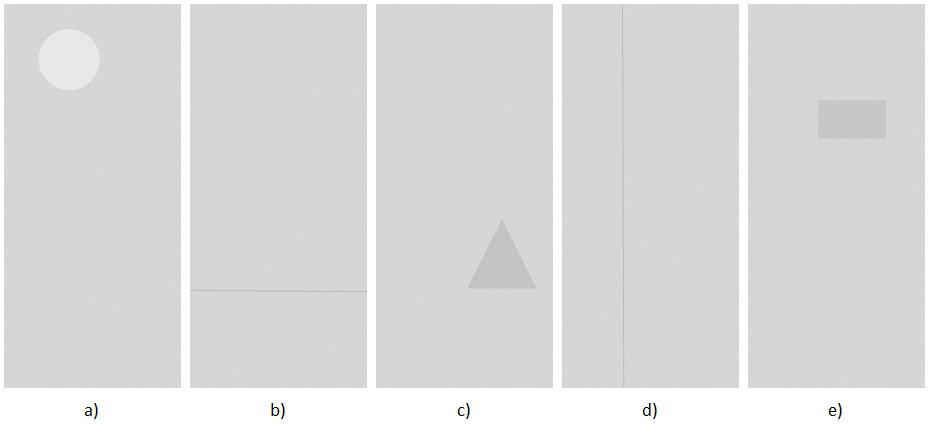
\includegraphics[width=0.85\linewidth]{figures/c4/c4_pattern.png}
    \caption{Năm dạng khuyết tật hình học bề mặt màn hình điện thoại trong tập dữ liệu thực nghiệm.}
    \label{fig:c4_pattern}
\end{figure}

\begin{figure}[htbp]
    \centering
    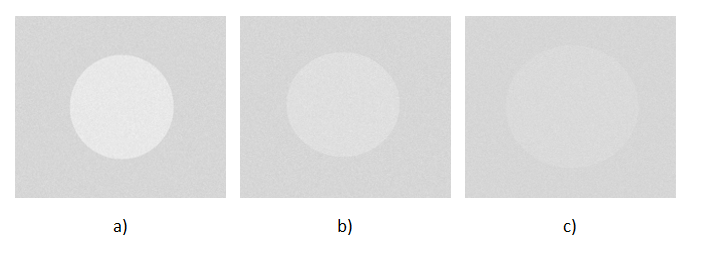
\includegraphics[width=0.75\linewidth]{figures/c4/c4_level_pattern.png}
    \caption{Ba cấp độ cường độ khuyết tật từ mạnh đến yếu đại diện cho dạng khuyết tật đường tròn.}
    \label{fig:c4_level_pattern}
\end{figure}

Dòng dữ liệu học trực tuyến được thiết lập dưới dạng chuỗi xuất hiện nối tiếp của năm loại khuyết tật qua năm giai đoạn liên tiếp nhằm tạo ra hiện tượng trôi dạt khái niệm đột ngột. Bảng \ref{tab:defect_summary} trình bày chi tiết sự phân bố mẫu, phạm vi chỉ số chuỗi dữ liệu và số lượng ảnh theo từng cấp độ cường độ khuyết tật. Mỗi loại khuyết tật đóng góp $600$ mẫu dữ liệu liên tục, trong đó mỗi cấp độ cường độ khuyết tật chiếm $200$ mẫu. Tại các mốc chuyển giao giữa các giai đoạn dữ liệu, sự thay đổi hoàn toàn của phân bố đặc trưng buộc thuật toán EAGNG phải thích ứng linh hoạt để tự động hình thành các nút biểu diễn mới mà không làm mất đi tri thức đã tích lũy từ các giai đoạn trước.

\begin{table}[htbp]
    \centering
    \caption{Thống kê chi tiết kịch bản phân bố dòng dữ liệu khuyết tật theo giai đoạn và cường độ.}
    \label{tab:defect_summary}
    \renewcommand{\arraystretch}{1.2}
    \begin{tabular}{|c|c|c|c|c|}
        \hline
        Giai đoạn & Loại khuyết tật & Cường độ khuyết tật & Phạm vi mẫu & Số lượng ảnh \\
        \hline
        1 & Đường tròn & Mạnh / Vừa / Yếu & 1--600 & 200 / 200 / 200 \\
        \hline
        2 & Đường ngang & Mạnh / Vừa / Yếu & 601--1200 & 200 / 200 / 200 \\
        \hline
        3 & Hình tam giác & Mạnh / Vừa / Yếu & 1201--1800 & 200 / 200 / 200 \\
        \hline
        4 & Đường dọc & Mạnh / Vừa / Yếu & 1801--2400 & 200 / 200 / 200 \\
        \hline
        5 & Hình chữ nhật & Mạnh / Vừa / Yếu & 2401--3000 & 200 / 200 / 200 \\
        \hline
    \end{tabular}
\end{table}